%! TeX root = ../charles/en/thesis.tex

\chapter{Background}
\label{chap:bg}

In this chapter, we briefly cover progress in obtaining useful representations
of language (Section \ref{sec:lm}), images (Section \ref{sec:imrec}), and
efforts to combine these two modalities (Section \ref{sec:vlm}). We then
discuss the extension of vision and language models to videos (Section
\ref{sec:vidlm}), which introduces the extra complexity of reasoning across
sequences of images, and optionally adding a further modality, audio. Finally,
we explore the literature on temporal reasoning in language and in vision
(Section \ref{sec:tempreason}).
%We finish the chapter with an introduction to and motivation for studying the
%task of video question answering (Section \ref{sec:vidqa}).

\section{Language Modeling}
\label{sec:lm}

Language modeling is the task of predicting a word given a previous token of
words. 


\subsection{Recurrent Neural Networks}
\label{ssec:rnn}

Vanilla RNN, LSTM, GRU, attention
	
\subsection{Transformer}
\label{ssec:transformer}

\cite{vaswani2017attention} introduced the Transformer architecture for
sequence tasks, replacing the recurrent nature of the RNN and its variants with
multi-head self-attention. Allows for parallel computation, but cost of
$O(n^2)$ in sequence length.

More recent implementations improve this, e.g. Flash Attention (maybe not relevant)

\section{Image Recognition}
\label{sec:imrec}

A key part of video and language models is learning representations of frames
in sequence, which involves the classical tasks of object detection,
segmentation, and image classification.

Object detection, classification

\subsection{Convolutional Neural Networks}
\label{ssec:cnn}

Convolutional neural networks (CNNs) such as
AlexNet~\citep{krizhevsky2012alexnet}, ResNet~\citep{he2016resnet},

\subsection{Vision Transformer}
\label{ssec:vit}

\cite{dosovitskiy2021vit} introduced the Vision Transformer (ViT), which takes
the impressive performance of the Transformer architecture on sequence tasks
and applies it to image tasks. The authors represent an image as a sequence of
patches of an image, with an extra patch embedding added alongside the
positional embedding of the Transformer \cite{vaswani2017attention} to maintain
the 2-dimensional information of an image when projected into a linear
sequence. 

\subsection{CLIP}
\label{ssec:clip}

\cite{radford2021clip} introduced CLIP (Contrastive Language-Image
Pre-training), which uses the Info-NCE loss~\citep{oord2019infonce} to jointly
learn relationships between encodings of text captions and extracted feature
representations of associated images. The Info-NCE loss trains a multimodal
embedding space to maximise the cosine similarity of matching pairs of captions
and images, while minimising the cosine similarity of non-matching pairs in the
batch. The approach is shown in Fig.~\ref{fig:clip}. A key part of this
approach is using a very large batch, so that there are many incorrect pairings
to learn from. \cite{radford2021clip} use a batch size of 32768. The text
encoder is a Transformer~\citep{vaswani2017attention}, and their best model
uses a Vision Transformer~\citep{dosovitskiy2021vit} as the image encoder.

\begin{figure}[htpb]
	\centering
	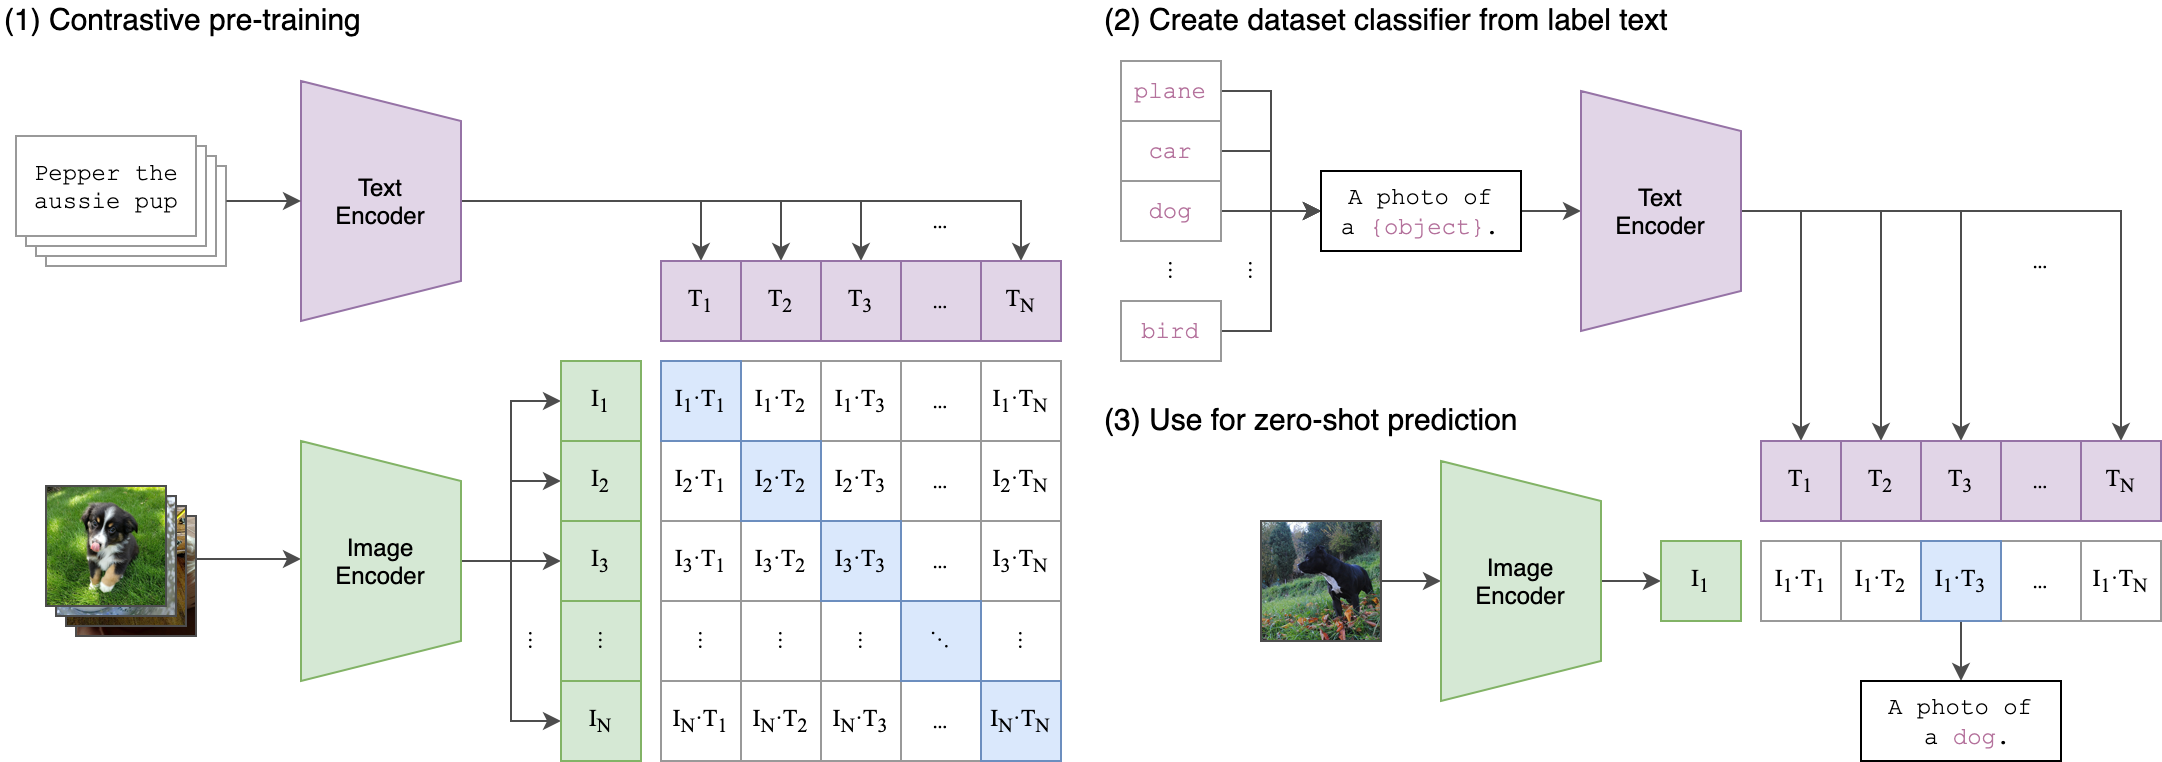
\includegraphics[width=\textwidth]{CLIP.png}
	\caption{CLIP. From~\cite{radford2021clip}}
	\label{fig:clip}
\end{figure}

The model enables zero-shot transfer to many downstream computer vision
classification tasks by predicting the most probable (image, text) pair when
given an image and a set of text prompts with each class embedded in the prompt
achieving performance comparable to or surpassing the previous state of the art
by finetuned models. The representations learned by the contrastive
pre-training objective have wide applicability to a range of VLM and Video
Language Models, particularly as frozen features from which to add smaller
modules on top for adapting to vision and language
tasks~\citep{alayrac2022flamingo,lin2022evl,lei2021clipbert}. We discuss some
of these models in Section~\ref{sec:vidlm}, and consider the limitations and
possible expansions of the contrastive pre-training method
in Section~\ref{sec:contrastive}.


\section{Vision and Language Models}
\label{sec:vlm}

One criticism of language models is that the representations learned by
training a model to predict the next word fails to learn any kind of
meaning~\citep{bender2020climbing} without reference to the real world. Models
trained in this way learn connections between surface forms, but no grounded
meaning between the form and intent portrayed through the form. A way to create
grounded representations may be to combine the two modalities of language and
vision through multimodal embeddings. A key challenge in recent years has been
to find suitable methods for creating these shared representations.

Following the success in NLP of BERT~\citep{devlin2019bert},
\cite{li2019visualbert} extends BERT to include visual features extracted from
a CNN as well as text tokens as input to a
Transformer~\citep{vaswani2017attention}, implicitly discovering a joint
representation between the two modalities. \cite{lu2019vilbert}

Other approaches take frozen encodings of image, text, or both, and learn a
shared embedding space on top of this (e.g. BLIP-2 \cite{li2023blip2})

Many approaches, joint training with concatenated image and text features into
BERT (VisualBERT), learning both image and text features concurrently.


\subsection{Visual Question Answering}
\label{ssec:vqa}

Datasets, multiple-choice vs open-ended

\section{Video Language Models}
\label{sec:vidlm}

Models which take as input video. How to choose frames, methods for learning
temporal aspect, modeling sequences of images

\subsection{Adapted from Vision and Language Models}
\label{sec:adaptvlm}

Models which take models trained on images and adapt to video

\cite{buch2022revisiting} -- Testing video tasks on single frames

\cite{wang2022vidil} -- VidIL (prompt engineering gives lists of objects,
events, attributes identified in frames, along with individual captions).
Language model (InstructGPT \cite{ouyang2022instructgpt}) left to produce
video-level captions, with specially designed prompts (``first\ldots then\ldots
finally''). No finetuning or pretraining on video

\cite{zeng2023socratic} -- Similar idea to VidIL

\subsection{Training on Videos}
\label{sec:vidtrain}

Models which take into account temporal nature and train/finetune on video datasets

\cite{lin2022evl} -- train video recognition models from frozen CLIP features

\section{Temporal Reasoning}
\label{sec:tempreason}

All about literature on temporal reasoning. From video perspective, from
language perspective

\cite{allen1983interval}
\cite{bruce1972temporalqa}
\cite{zhou2021tracie}

%\section{Video Question Answering}
%\label{sec:vidqa}
%
%\subsection{STAR Dataset}
%\label{ssec:star}
%
%We primarily focus on this due to its focus on sequential questions that evaluate model performance on temporal reasoning
%
%\subsection{Merlot Reserve}
%\label{ssec:mreserve}
%
%We examine a specific video language model, Merlot Reserve \citep{zellers2022mreserve}, that performs strongly on STAR.
